% Report of results from Ramsay simulation experiment
% David Lawrence Miller
% d.l.miller@bath.ac.uk

% Started : 8th April 2009

\documentclass[a4paper,10pt]{amsart}

% Load some packages
\usepackage{times, amsmath, amssymb, amsfonts, url, natbib, bm, rotating,multirow,graphicx}

% top matter
\title{Smoothing over irregular shapes using the Schwarz-Christoffel transform}
\author{David Lawrence Miller}
\email{d.l.miller@bath.ac.uk}
\address{Mathematical Sciences, University of Bath, Bath, United Kingdom}

% Shortcuts
% Probability
\newcommand{\prob}[1]{\mathbb{P}\left[ #1 \right]}
% Hovitz-Thompson
\newcommand{\HT}{\hat{\tau}_{HT}}
% Schwarz-Christoffel
\newcommand{\sch}{Schwarz-Christoffel }
% fprime
\newcommand{\fprime}{f^\prime(z)}
% figure reference command
\newcommand{\fig}[1]{\emph{fig.} (\ref{#1})}
% figure reference command (start of sentance
\newcommand{\Fig}[1]{\emph{Fig.} (\ref{#1})}
% equation reference command
\newcommand{\eqn}[1]{\emph{eqn.} (\ref{#1})}
% phi inverse
\newcommand{\phiinv}{\phi^{-1}}
% use other phi
\newcommand{\ophi}{\phi}
\renewcommand{\phi}{\varphi}




\begin{document}

% The abstract
\begin{abstract}
Following on from looking at the Ramsay horseshoe, other polygon mappings are simulated from and transformed with the \sch transform.
\end{abstract}


% New theorem for theorems
\newtheorem{thm}{Theorem}[section]

%New theorem for definitions
\newtheorem{defn}{Definition}[section]

\maketitle



\section{Looking at other domains}

Given the relative success of using the \sch transform on the Ramsay horseshoe, and the relative failure of using it on the alternate Ramsay horseshoe, more conclusive evidence is needed to investigate the properties of the transform and its utility to smoothing over complex regions.





\section{General setup}

For all of the examples below the function \texttt{mvnorm} from the \textsf{R} package \texttt{MASS} was used to generate a surface over the region in question made up of multivariate Normal distributions. This was then discretized over a 50x50 grid. A 500 replicate simulation was then run at two noise levels ($\sigma^2=0.02$, $\sigma^2=0.005$) and two sample sizes (1000, 500.) For each replicate we fit a model with thin plate regression splines, the soap film smoother of \cite{soap} and finally thin plate regression splines on the \sch transformed domain.






\section{Example 1}

We begin with an example from \cite{miller09}, which is shown in \ref{fig9}. We used the SC Toolbox for MATLAB to map the figure to both the unit disk and rectangle.

\begin{figure}
\centering
% trim order l b r t
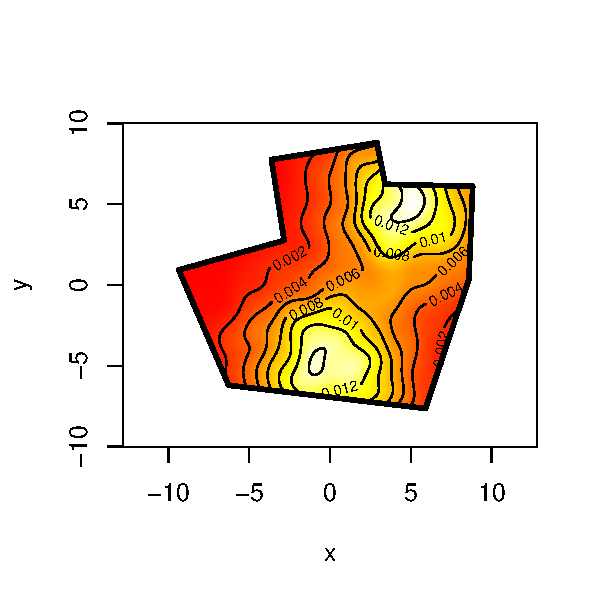
\includegraphics[width=2in]{figs-otherdomains/fig9.png} \\
\caption{The heatmap of the polygon's generated density.}
\label{fig9}
% generated by /phd-smoothing/sc-writeup/figs-otherdomains/fig9.R
\end{figure}

\subsection{Unit disk}

\Fig{fig9-disk-real} shows an example fit for the three methods along with the true surface when the region is deformed to the unit disk. Results of the simulations are summarized in table \ref{fig9-disk-table} and the boxplots in \fig{fig9-disk-boxplots}. From this we can see that the thin plate regression splines appear to do very well for all cases, with the methods equaling out with a smaller sample size.

\begin{figure}
\centering
% trim order l b r t
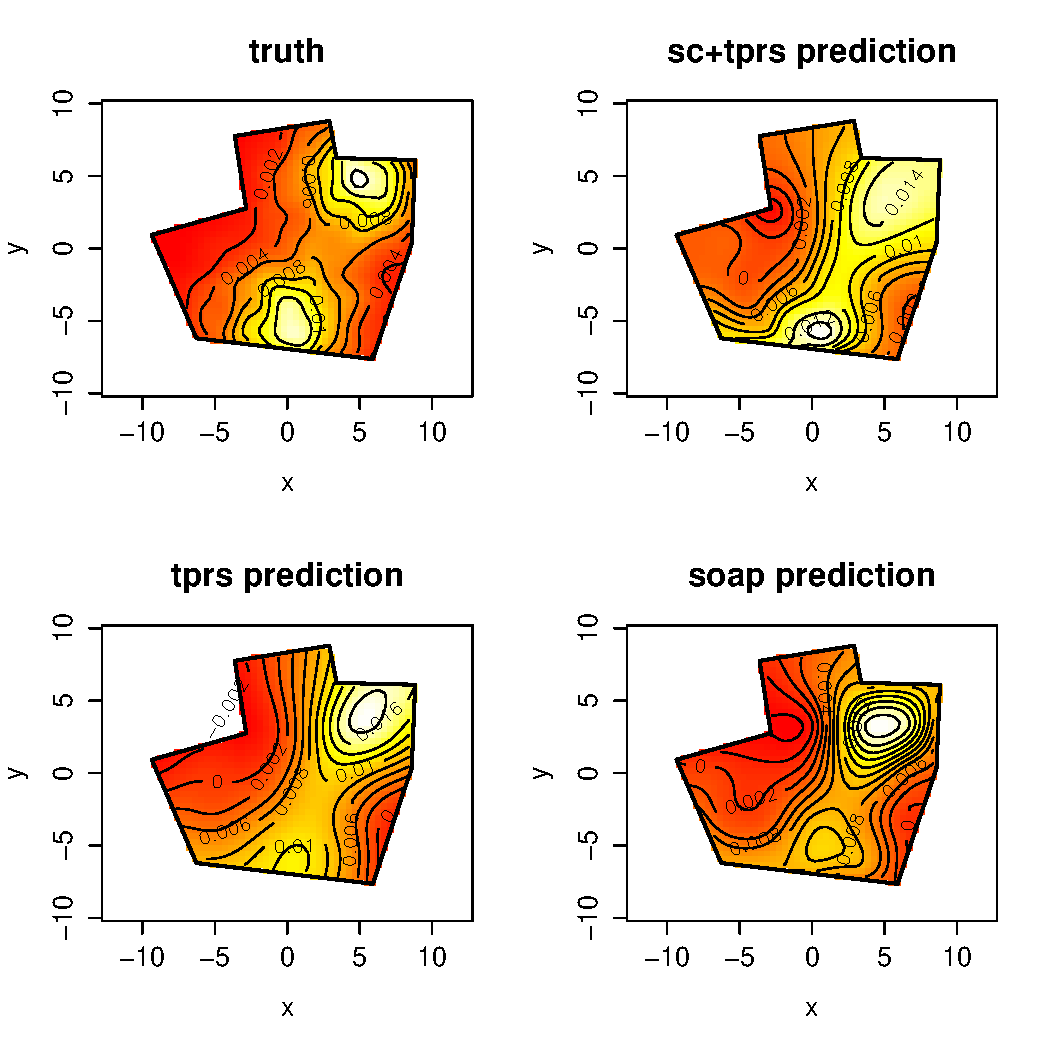
\includegraphics[width=3in]{figs-otherdomains/fig9-disk-real.pdf} \\
\caption{Truth and fits from one realization when there was a sample size of 500 and the noise level was set to 0.02 when the shape was deformed to the unit disk. }
\label{fig9-disk-real}
% generated by fig9test/fit.irregular.R
\end{figure}


\begin{table}[ht]
\begin{tabular}{c c c c c}\\
Method & Noise level & Sample size & MSE & se(MSE)\\
\hline
\hline
SC+TPRS & 0.02 & 1000 & 1.1451e-05 & 3.7161e-06\\
TPRS & 0.02 & 1000 & 9.0171e-06 & 3.6261e-06\\
soap & 0.02 & 1000 & 1.0998e-05 & 5.2048e-06\\
SC+TPRS & 0.005 & 1000 & 1.9542e-06 & 3.7125e-07\\
TPRS & 0.005 & 1000 & 1.2578e-06 & 3.0429e-07\\
soap & 0.005 & 1000 & 1.47e-06 & 3.8266e-07\\
SC+TPRS & 0.02 & 500 & 1.7449e-05 & 6.4406e-06\\
TPRS & 0.02 & 500 & 1.5523e-05 & 7.1658e-06\\
soap & 0.02 & 500 & 1.8678e-05 & 1.2239e-05\\
SC+TPRS & 0.005 & 500 & 3.1202e-06 & 7.4002e-07\\
TPRS & 0.005 & 500 & 2.1378e-06 & 6.2306e-07\\
soap & 0.005 & 500 & 2.7517e-06 & 2.0487e-06\\
\end{tabular}
\caption{The mean squared error and its standard error for 500 realizations of example 1.}
\label{fig9-disk-table}
\end{table}

[WHY?!]

\begin{figure}[p]
\centering
% trim order l b r t
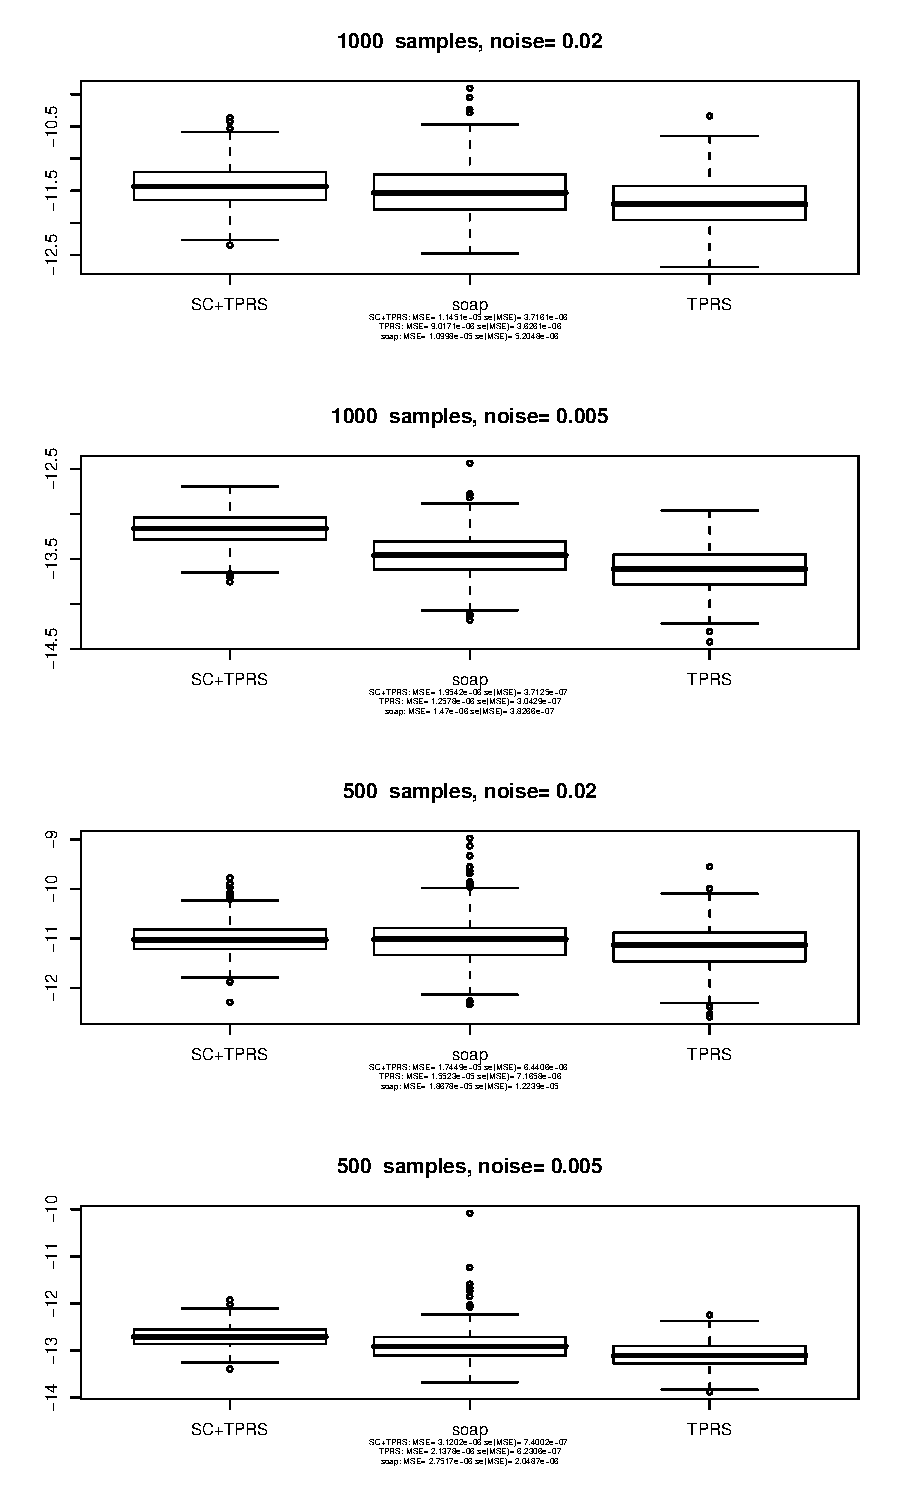
\includegraphics[width=5in]{figs-otherdomains/fig9-disk-boxplot.pdf} \\
\caption{Boxplot of mean squared error per prediction point over 500 replicates for the unit disk mapping for example 1. }
\label{fig9-disk-boxplots}
% generated by fig9test/makeboxplots.R
\end{figure}


\subsection{Rectangle}

We then repeat the process using the rectangular mapping, vertices chosen (somewhat arbitrarily) to map to those of the rectangle were 1, 6, 8 and 9 (see \fig{fig9-numbered}.)


\begin{figure}
\centering
% trim order l b r t
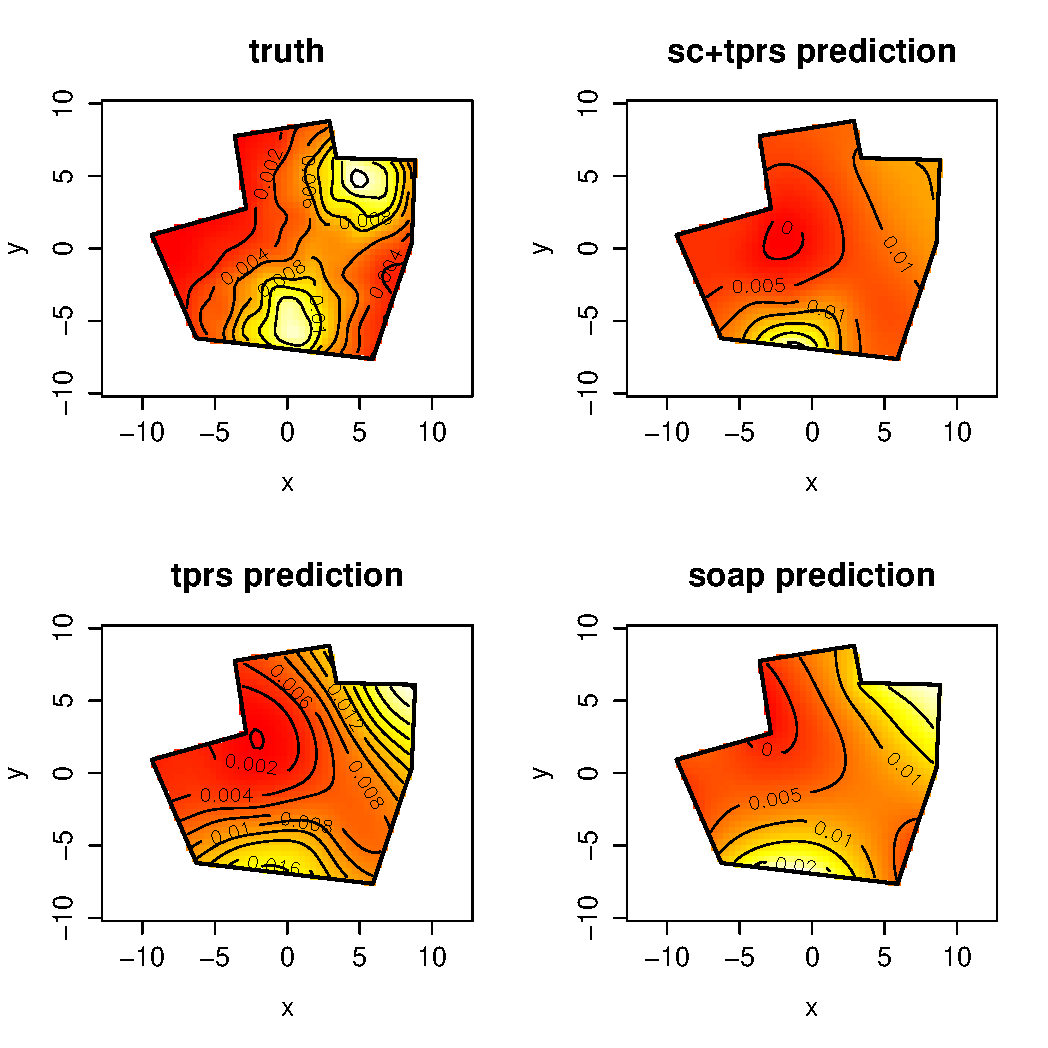
\includegraphics[width=3in]{figs-otherdomains/fig9-rect-real.pdf} \\
\caption{Truth and fits from one realization when there was a sample size of 500 and the noise level was set to 0.02 when the rectangular mapping was used. }
\label{fig9-rect-real}
% generated by fig9test/fit.irregular.R
\end{figure}

\begin{figure}
\centering
% trim order l b r t
\includegraphics[width=2in]{figs-otherdomains/fig9-numbered.png} \\
\caption{Vertex numbering for the first example.}
\label{fig9-numbered}
% generated by Matlab
\end{figure}


\begin{table}[ht]
\begin{tabular}{c c c c c}\\
Method & Noise level & Sample size & MSE & se(MSE)\\
\hline
\hline
SC+TPRS & 0.02 & 1000 & 1.1541e-05 & 3.4491e-06\\
TPRS & 0.02 & 1000 & 9.2969e-06 & 3.8674e-06\\
soap & 0.02 & 1000 & 1.1457e-05 & 5.9093e-06\\
SC+TPRS & 0.005 & 1000 & 1.9252e-06 & 3.735e-07\\
TPRS & 0.005 & 1000 & 1.2603e-06 & 3.3009e-07\\
soap & 0.005 & 1000 & 1.4676e-06 & 4.1855e-07\\
SC+TPRS & 0.02 & 500 & 1.7332e-05 & 6.7812e-06\\
TPRS & 0.02 & 500 & 1.5592e-05 & 7.654e-06\\
soap & 0.02 & 500 & 1.8546e-05 & 1.1888e-05\\
SC+TPRS & 0.005 & 500 & 3.0787e-06 & 6.625e-07\\
TPRS & 0.005 & 500 & 2.085e-06 & 5.4026e-07\\
soap & 0.005 & 500 & 2.5785e-06 & 1.2369e-06\\
\end{tabular}
\caption{The mean squared error and its standard error for 500 realizations of example 1.}
\label{fig9-rect-table}
\end{table}



\begin{figure}[p]
\centering
% trim order l b r t
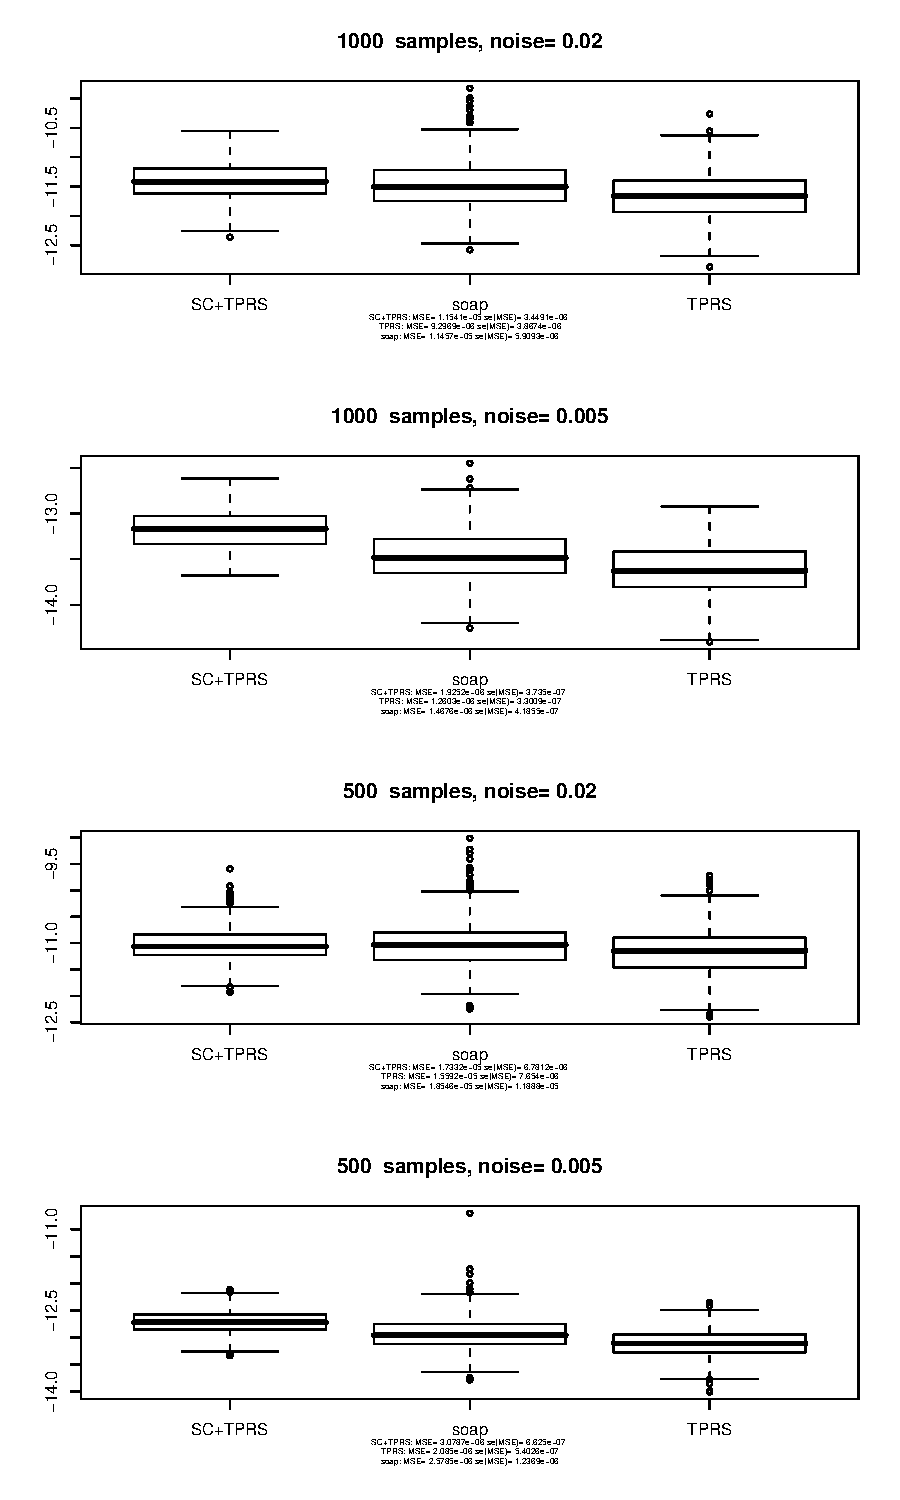
\includegraphics[width=5in]{figs-otherdomains/fig9-rect-boxplot.pdf} \\
\caption{Boxplot of mean squared error per prediction point over 500 replicates for the rectangle mapping for example 1. }
\label{fig9-rect-boxplots}
% generated by fig9test/makeboxplots.R
\end{figure}








\section{Example 2}


which vertices were numbered?

\begin{figure}
\centering
% trim order l b r t
\includegraphics[width=2in]{figs-otherdomains/wigglytop-numbered.png} \\
\caption{Vertex numbering for the second example.}
\label{wigglytop-numbered}
% generated by Matlab
\end{figure}






\begin{table}[ht]
\begin{tabular}{c c c c c}\\
Method & Noise level & Sample size & MSE & se(MSE)\\
\hline
\hline
SC+TPRS & 0.02 & 1000 & 4.4262e-05 & 5.653e-06\\
TPRS & 0.02 & 1000 & 1.973e-05 & 4.8263e-06\\
soap & 0.02 & 1000 & 2.6918e-05 & 5.7648e-06\\
SC+TPRS & 0.005 & 1000 & 2.1901e-05 & 1.0675e-06\\
TPRS & 0.005 & 1000 & 3.7205e-06 & 5.1288e-07\\
soap & 0.005 & 1000 & 6.4839e-06 & 8.3582e-07\\
SC+TPRS & 0.02 & 500 & 6.1488e-05 & 1.1247e-05\\
TPRS & 0.02 & 500 & 3.256e-05 & 9.327e-06\\
soap & 0.02 & 500 & 4.416e-05 & 1.2662e-05\\
SC+TPRS & 0.005 & 500 & 2.5596e-05 & 2.3287e-06\\
TPRS & 0.005 & 500 & 5.9221e-06 & 1.0344e-06\\
soap & 0.005 & 500 & 1.0391e-05 & 3.4061e-06\\
\end{tabular}
\caption{The mean squared error and its standard error for 500 realizations of example 2.}
\label{wigglytop-table}
\end{table}

% boxplot
\begin{figure}[p]
\centering
% trim order l b r t
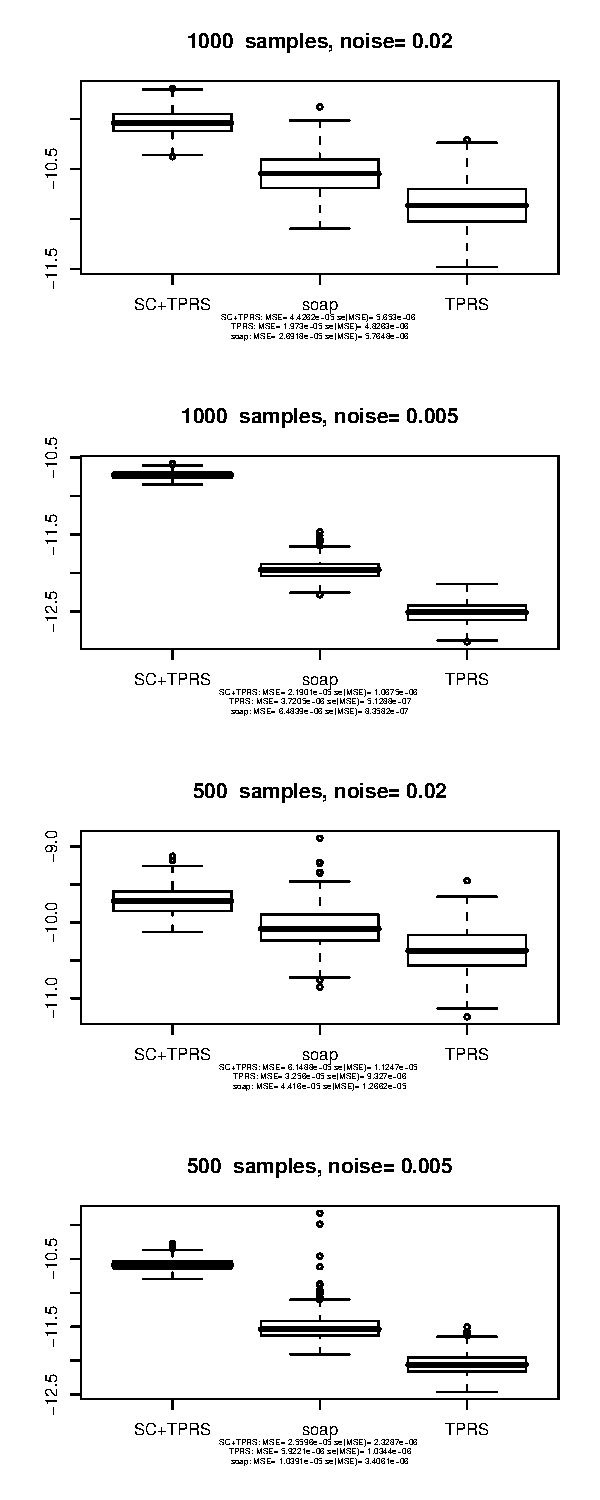
\includegraphics[width=3in]{figs-otherdomains/wigglytop-boxplot.pdf} \\
\caption{Boxplot of mean squared error per prediction point over 500 replicates for the rectangle mapping for example 2. }
\label{wigglytop-boxplots}
% generated by makeboxplots.R
\end{figure}


% realization
\begin{figure}
\centering
% trim order l b r t
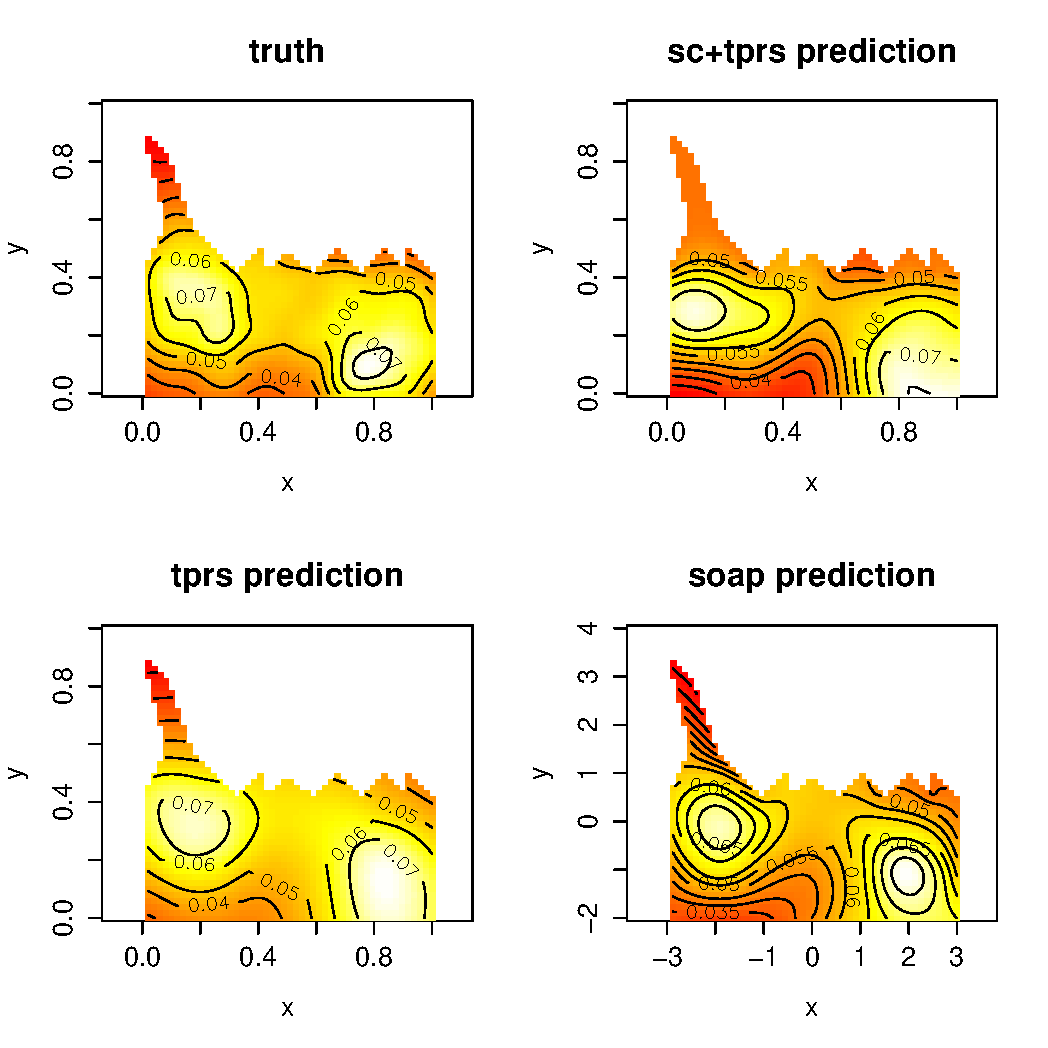
\includegraphics[width=3in]{figs-otherdomains/wigglytop-real.pdf} \\
\caption{Truth and fits from one realization when there was a sample size of 500 and the noise level was set to 0.02 when the rectangular mapping was used for example 2. }
\label{wigglytop-real}
% generated by wigglytop fit.irregular.R
\end{figure}




\section{Example 3}

We repeated the procedure for another polygon with two peninsulae, shown in \fig{wigglytop2dia}. Initially, a transform using \texttt{rectmap} was used, but this failed to converge, so \texttt{crrectmap} was used.

\begin{figure}
\centering
% trim order l b r t
\includegraphics[width=2in]{figs-otherdomains/wigglytop2-numbered.png} \\
\caption{CRDT pic. EXPLAIN}
\label{wigglytop2-numbered}
% generated by Matlab
\end{figure}

\begin{table}[ht]
\begin{tabular}{c c c c c}\\
Method & Noise level & Sample size & MSE & se(MSE)\\
\hline
\hline
SC+TPRS & 0.02 & 1000 & 0.0088323 & 0.00022266\\
TPRS & 0.02 & 1000 & 0.0024431 & 0.00048805\\
soap & 0.02 & 1000 & 0.0018471 & 0.0014468\\
SC+TPRS & 0.005 & 1000 & 0.0088005 & 0.0002257\\
TPRS & 0.005 & 1000 & 0.0023752 & 0.00048408\\
soap & 0.005 & 1000 & 0.0017429 & 0.0014925\\
SC+TPRS & 0.02 & 500 & 0.0095545 & 0.00047307\\
TPRS & 0.02 & 500 & 0.0030897 & 0.00091674\\
soap & 0.02 & 500 & 0.017676 & 0.071426\\
SC+TPRS & 0.005 & 500 & 0.0095272 & 0.00047354\\
TPRS & 0.005 & 500 & 0.0029209 & 0.00084832\\
soap & 0.005 & 500 & 0.019301 & 0.10139\\
\end{tabular}
\caption{example 3}
\label{}
\end{table}

% boxplot
\begin{figure}[p]
\centering
% trim order l b r t
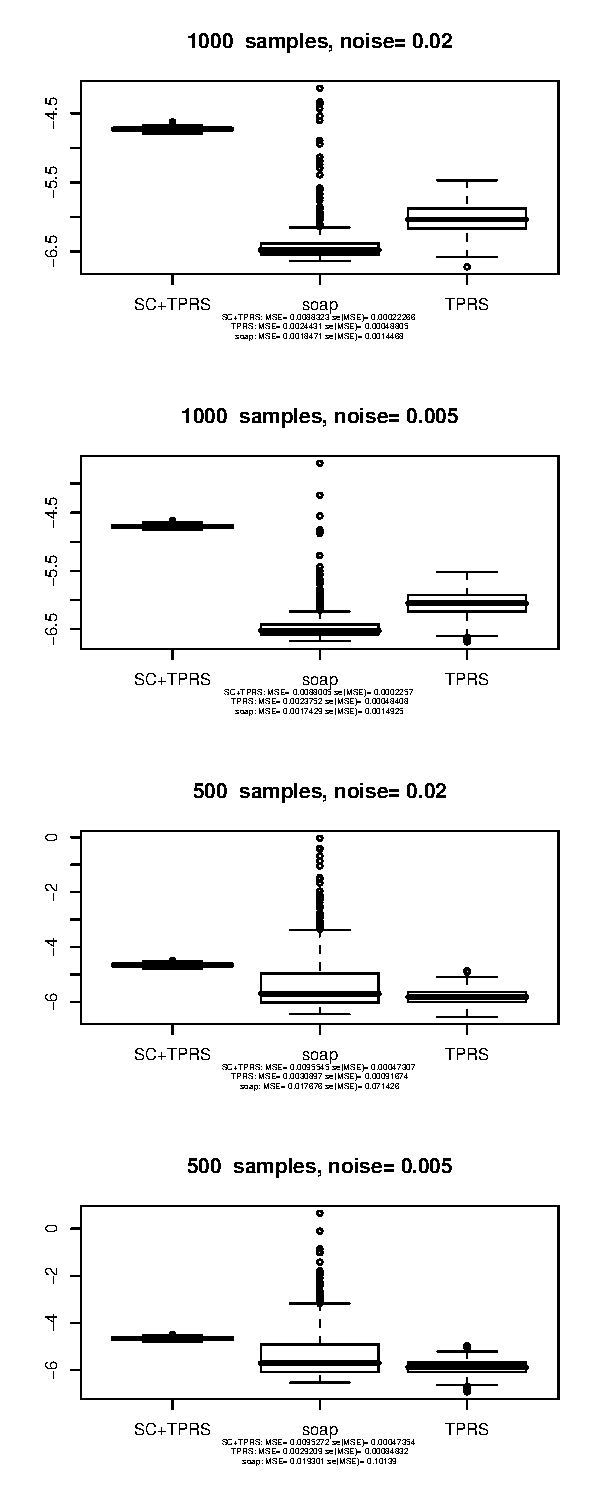
\includegraphics[width=3in]{figs-otherdomains/wigglytop2-boxplot.pdf} \\
\caption{Boxplot of mean squared error per prediction point over 500 replicates for the rectangle mapping for example 3. }
\label{wigglytop2-boxplots}
% generated by makeboxplots.R
\end{figure}


% realization
\begin{figure}
\centering
% trim order l b r t
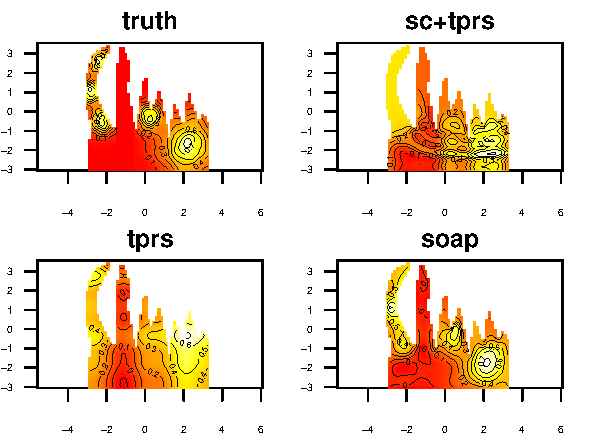
\includegraphics[width=3in]{figs-otherdomains/wigglytop2-real.pdf} \\
\caption{Truth and fits from one realization when there was a sample size of 500 and the noise level was set to 0.02 when the rectangular mapping was used for example 3. }
\label{wigglytop2-real}
% generated by wigglytop2 fit.irregular.R
\end{figure}

%%%%%%%%%%%%%%%%%%% bounding box
\section{Example 4}

Using a bounding box


\begin{figure}
\centering
% trim order l b r t
\includegraphics[width=2in]{figs-otherdomains/wigglytop2-bbox-numbered.png} \\
\caption{CRDT pic. EXPLAIN}
\label{wigglytop2-bbox-numbered}
% generated by Matlab
\end{figure}




\begin{table}[ht]
\begin{tabular}{c c c c c}\\
Method & Noise level & Sample size & MSE & se(MSE)\\
\hline
\hline
SC+TPRS & 0.02 & 1000 & 0.012993 & 0.0010068\\
TPRS & 0.02 & 1000 & 0.0022156 & 0.0003959\\
soap & 0.02 & 1000 & 0.0028811 & 0.011293\\
SC+TPRS & 0.005 & 1000 & 0.012856 & 0.0010157\\
TPRS & 0.005 & 1000 & 0.0021704 & 0.00039474\\
soap & 0.005 & 1000 & 0.0020087 & 0.0082462\\
SC+TPRS & 0.02 & 500 & 0.012305 & 0.0014609\\
TPRS & 0.02 & 500 & 0.0027819 & 0.00069713\\
soap & 0.02 & 500 & 0.11246 & 1.8866\\
SC+TPRS & 0.005 & 500 & 0.012316 & 0.0015265\\
TPRS & 0.005 & 500 & 0.0027275 & 0.00070468\\
soap & 0.005 & 500 & 0.38048 & 4.358\\
\end{tabular}
\caption{}
\label{example 4}
\end{table}

% boxplot
\begin{figure}[p]
\centering
% trim order l b r t
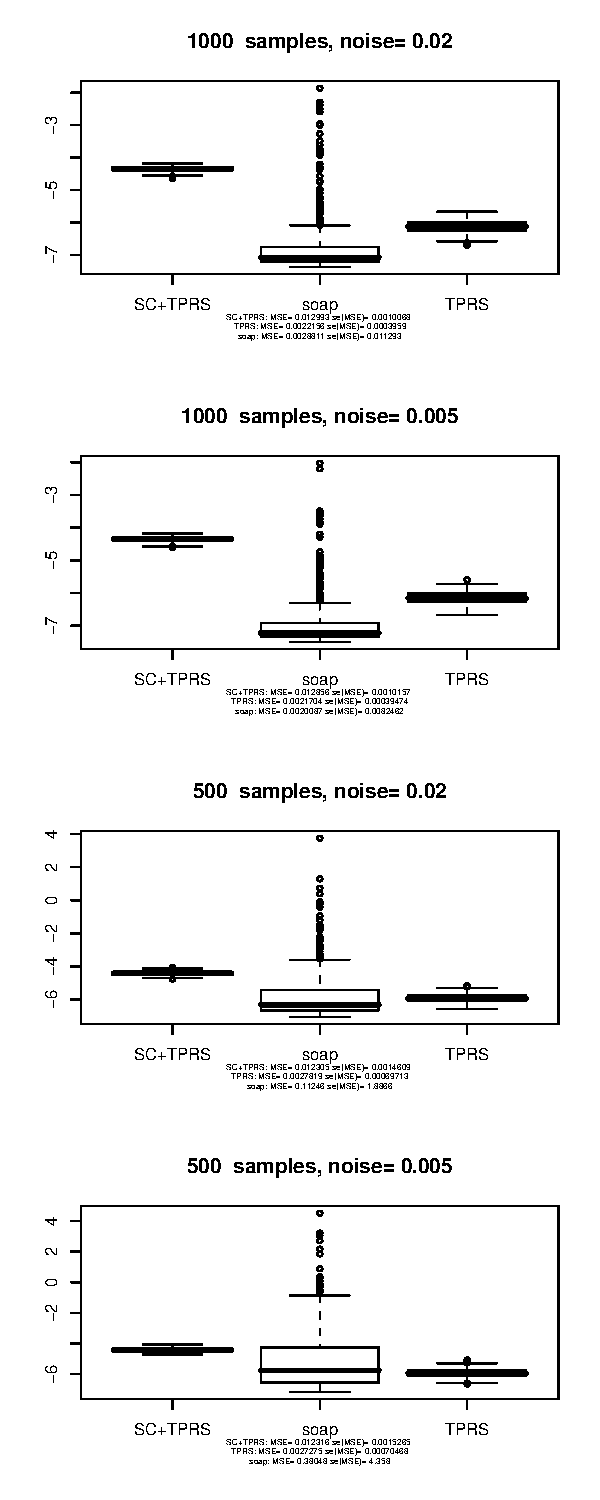
\includegraphics[width=3in]{figs-otherdomains/wigglytop2-bbox-boxplots.pdf} \\
\caption{Boxplot of mean squared error per prediction point over 500 replicates for the rectangle mapping for example 4.}
\label{wigglytop2-bbox-boxplots}
% generated by makeboxplots.R
\end{figure}


% realization
\begin{figure}
\centering
% trim order l b r t
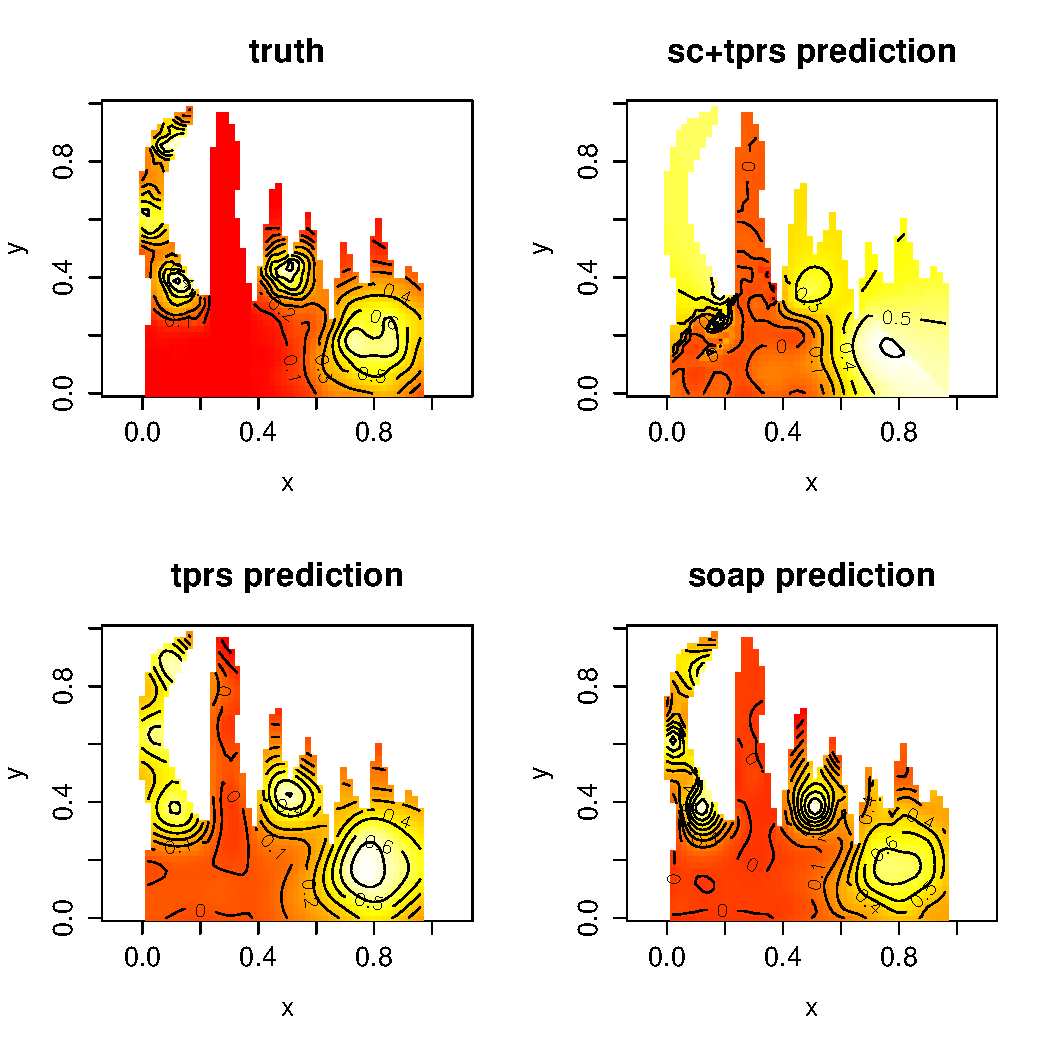
\includegraphics[width=3in]{figs-otherdomains/wigglytop2-bbox-real.pdf} \\
\caption{Truth and fits from one realization when there was a sample size of 500 and the noise level was set to 0.02 when the rectangular mapping was used for example 4.}
\label{wigglytop2-bbox-real}
% generated by wigglytop2-bbox fit.irregular.R
\end{figure}


\section{Conclusion}

This is rubbish.

Arbitrary vertex choice.

SQuashing of the features in wigglytop case.












\bibliographystyle{plainnat}
\bibliography{sc-refs}



\end{document}
